% find this class at https://archive.danleonard.us/scholarship/coursework/coursework.cls
\documentclass[american]{../../../coursework}

\title{Water Security of Arctic Peoples}
\subtitle{}
\author{Daniel}{Glenn}{Leonard}
\newdate{date}{11}{05}{2017}
\date{\displaydate{date}}
\course{ESE}{320}{Water Planet, Water Crisis}{University of Illinois at Urbana-Champaign}
\instructor{Dr}{Murugesu}{}{}{Sivapalan}

\keywords{}
\addbibresource{arctic.bib}
%\addbibresource[location=remote]{https://archive.danleonard.us/scholarship/coursework/illinois/ESE/320/arctic.bib}
\baseurl{https://archive.danleonard.us/scholarship/coursework/illinois/ESE/320/arctic.xhtml}

\begin{document}

\maketitle

Arctic peoples, especially indigenous subsistence hunters, are often
overlooked when it comes to the global water crisis. Although some may have
been surviving on ice for thousands of years, many communities are still
subject to poor infrastructure and are especially affected by global climate
change. Solutions to these crises depend strongly on region, with soft-path
rainwater harvesting working in some subarctic communities but others
requiring hard-path infrastructure such as piped running water.

The Millennium Development Goals of the United Nations~(UN) are targets that
include the access to clean water for everyone on Earth. For good reason,
programs to help in the achievement of these focus on less-developed nations,
where the eight Arctic countries are all considered developed due to their
expansive southern populations. However, the polar areas of these countries
contain marginalized communities with low access to clean water that would not
qualify as meeting the UN's targets, the \enquote{fourth world}.

Many homes in rural Alaska do not have piped water service. Without such
service, people there must get water directly from the environment or from
stores which charge a high price for the service of transporting it. Thus,
these households, on average, only use 5.7~liters per person per day
\parencite{Hennessy2016}, what the World Health Organization considers
\enquote{no access} and of \enquote{very high} health concern
\parencite{Howard2003}. Doctors with the Alaskan Centers for Disease Control
have noted that Alaskan Native children have some of the world's highest rates
of invasive pneumococcal disease, even after introduction of the PCV7 vaccine.
The researchers strongly connect this problem to a lack of running water in
the homes of these children which limits handwashing \parencite{Wenger2010}.

In the Labrador town of Black Tickle, the Inuit residents must retrieve water
from shallow wells in town or from a small brook twenty-five kilometers away.
Counterintuitively, winter is the easiest season to retrieve water, as
traditional Inuit sleds allow for quick and easy travel. In the spring,
however, the ground is so wet that inhabitants must carry water on their
backs. As a result, nearly every man in the town reports chronic back and
shoulder pain and cannot undergo surgery as they are needed daily to procure
water. When the relatively new provincial water filtration system broke down
in 2012, the community saw an outbreak of gastrointestinal illness. Many older
members of the community have said that illness was a normal condition of the
town in the past \parencite{Hanrahan2014}.

Indigenous peoples of Siberia have lived there for much longer than those of
the New World, but they still suffer from the many problems of all Arctic
peoples. Researchers have surveyed the saturation of hot running water to
homes within all of Russia's regions. In Eastern Chukotka, the indigenous home
of Chukchi people, only 30\% of communities across the region had any access
to hot water \parencite{Hennessy2016}. It should be noted that access to
running water, even if hot, is safe for human use. In Arctic and Siberian
regions, centralized surface water sources have extreme levels of
contamination by both chemicals and biological agents. The study found over
50\% of sources had chlorine or magnesium, and nearly 1\% of water contained
Rotavirus or \emph{Clostridium} spores \parencite{Dudarev2013}. The water
crisis involves more than just drinking water. Drastic health impacts result
from lack of modern sewerage. The United Nations has noted that only 25-50\%
of housing in Nenets Autonomous Okrug has sewerage installed \parencite{2007},
and this is likely to be far more severe in the rural parts of the federal
subject.

Indigenous people of the Arctic are overwhelmingly subsistence hunters, and
for the Inuit, hunting is an important coming-of-age milestone. In North
America, the melting of sea ice in spring heralds the return of narwhal, whose
skin contains the greatest concentration of Vitamin C in the Arctic. Without
the narwhal, it's unlikely that the Inuit would have ever survived in much of
their territory \parencite{Brown2011}.

\begin{wrapfigure}{r}{0.5\textwidth}
    \begin{center}
        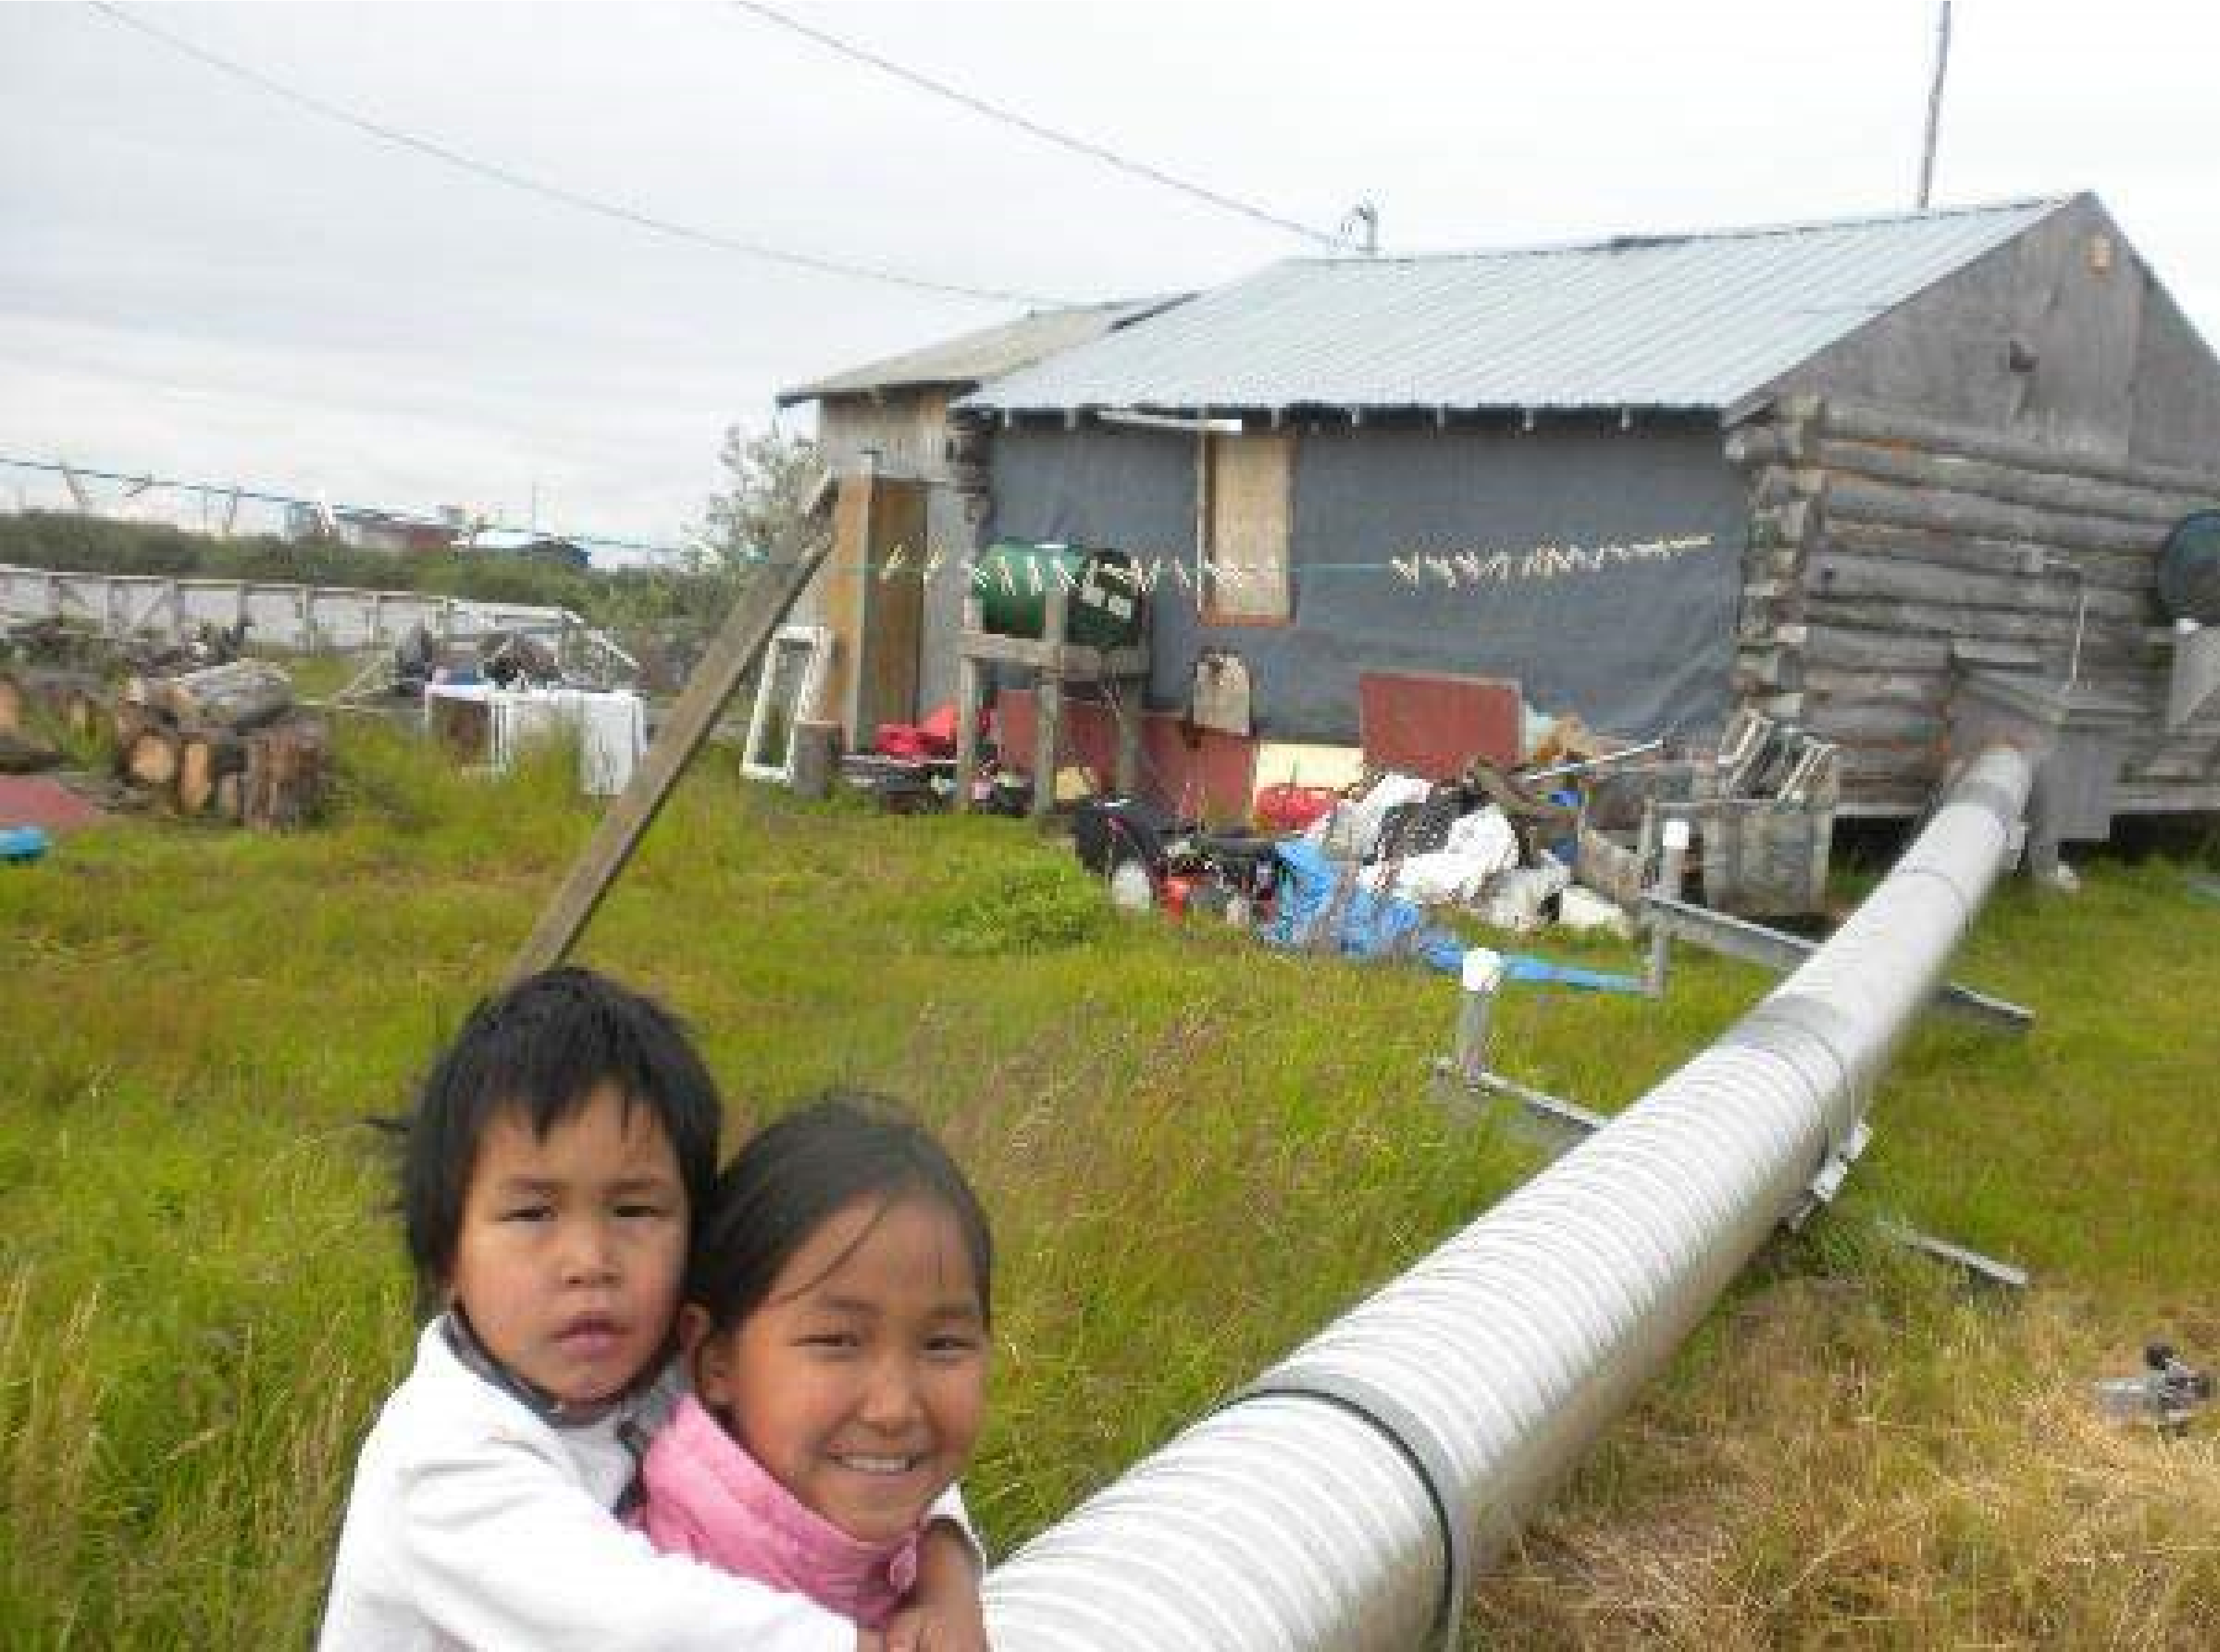
\includegraphics[width=0.48\textwidth]{arctic_photo.png}
%        \includegraphics[width=0.48\textwidth]{mbdtf.jpg}
    \end{center}
    \caption{A collapsed service line due to permafrost thaw in Selawik.
    Reprinted from \fullcite{Brubaker2016}. Copyright \citeyear{Brubaker2016}
    by \citeauthor{Brubaker2016}}%
    \label{fig:photo}
\end{wrapfigure}

Climate change is causing Arctic sea ice to melt drastically faster than it
had previously. Weakened sea ice prevents hunters from going out as far as in
past decades, as the ice can crack underfoot and subject the hunter to a
hypothermic plunge \parencite{Brown2011}. In 2013, two Inuit communities were
forced to cut short their hunting seasons after sea ice melted early and, as a
consequence, the Governor of Alaska declared them disaster areas. After the
ice melted even earlier the next year, the state government flew in
10,000~pounds of fish to save the communities \parencite{Struzik2016}.

In one Inuit village, hunting means scouring for mussels. Normally impossible 
with the permanent cover of ice, the community of Kangiqsujuaq breaks into
caverns under the sea ice, where the tide varies an incredible twelve meters.
There, they scour the exposed ocean floor for mollusks for a half hour until
the tide returns \parencite{Brown2011}. Rising ocean levels threaten to
shorten the gap between sea and land ice, possibly leading to such caverns
being permanently submerged. Without mussels, the residents of Kangiqsujuaq
will go without a major source of nutrition.

In the northwest Alaskan island of Kivalina, the community shares a single
facility with running water for showers, laundry, and toilets. A report by the
regional Department of Community Health Services discovered that since 2004,
storm surges resulting from lack of ice formation have caused this facility to
close frequently for extended periods. The sudden lack of flush toilets has
resulted in drastic health impacts, with increases in visits to the community
clinic for soft tissue infections \parencite{Thomas2013}.

While those in temperate regions are terrified of their pipes freezing and
breaking, those in the Arctic experience the opposite: thaw of permafrost can
allow the ground to shift and collapse infrastructure, especially
long-distance water piping (see Figure~\ref{fig:photo}). Climate change
threatens to exacerbate this damage. As permafrost melts deeper into the
Arctic Circle, more hard-path infrastructure will suffer severe damage.

Improving water access amongst Northern communities varies considerably on
local environments. Some locations, especially in the subarctic, have enough
rainfall or partially thawed lakes to provide some freshwater. In colder and
drier parts of the Arctic, it is unlikely that such easy acquisition of water
can be reliably obtained.

The Sustainable-Development Working Group~(SDWG) in the Arctic Council has
been working to discover new ways to sustainably provide in-home water and
sanitation to underserved Arctic communities. At the impending 10th
Ministerial Meeting of the Arctic Council on May 11, the foreign ministers of
Arctic nations are set to discuss the findings of the SDWG's 2016 Conference
on Water Innovations for Healthy Arctic Homes~(WIHAH).

\begin{figure}
    \begin{center}
        
\includegraphics[width=0.85\textwidth]{arctic_infographic.eps}
    \end{center}
    \caption{The Alaska Native Tribal Health Consortium's proposal for the
    State of Alaska Water \& Sewer Challenge Project. Reprinted from
    \fullcite[86]{PASS}. Copyright \citeyear{PASS} by \citeauthor{PASS}}%
    \label{fig:infographic}
\end{figure}

Across the Arctic, soft-path solutions are preferred. All Arctic nations,
especially Canada, decentralize their water distribution networks to the
community level, creating a great barrier for dispersed communities to access
water in the same way as Southern urban areas. Furthermore, some Arctic people
are wisely averse to drinking groundwater. Surveyed Inuit communities in
Alaska have noted a traditional preference for drinking snowmelt, especially
in winter, when it can be caught in buckets \parencite{Dotson2016}. Thus,
decentralized water services such as domestic rainwater harvesting and using
high-efficiency utilities can manage water effectively.

In the subarctic, rainwater harvesting can be a lucrative supplement to a
community's current source of water. In one particular Inuit community,
researchers implemented a pilot scheme that returned an average of
19.07~gallons of water weekly. The researchers noted that the rainwater was
not potable, and as such, drinking water did not increase; however, the
participants in the program testified that they felt healthier
\parencite{Mercer2017}. With improved water filtration, domestic rainwater
harvesting can be able to meet drinking water needs as well.

In Black Tickle, Labrador, researchers from the province's university trained
two locals to monitor the water sources for sanitation and send regular water
samples to Happy Valley-Goose Bay, the nearest large town
\parencite{Hanrahan2014}. Programs such as this can be extremely useful in
preventing disease before outbreaks occur. With so many in Black Tickle and
across the Arctic suffering from regular gastrointestinal sickness, it is
imperative that programs to monitor water quality are put in place across the
region.

The WIHAH conference included coverage of the Alaska Water and Sewer
Challenge, a state competition for engineers to design decentralized soft-path
solutions to poor sanitation. Currently, the program is in Stage 3 --
prototyping and lab testing the grant recipients. Most teams designed a system
with reverse-osmosis filtration to accompany waterless urinals, low-flow
sinks, and separating toilets (see Figure~\ref{fig:infographic}). This
drastically reduces water consumption while still allowing residents to
consistently use sanitary systems. A team from the University of Alaska
successfully designed a treatment system that, when coupled with a dry-flush
toilet, took eight weeks before needing to refill the water tank
\parencite{Dotson2016}.

With such severe problems in Arctic communities, it's shocking that they exist
within developed nations. It is imperative that soft-path solutions be
implemented to promote regional health and welfare. Thankfully, the Arctic
Council is working toward these goals with research grants and
interdisciplinary approaches. Domestic rainwater harvesting and
high-efficiency water reuse systems are extremely helpful to improve public
water access in the home, and teaching communities how to ensure their own
safety is beneficial in both promoting health and promoting indigenous
people's self-determination. However, climate change threatens the future
stability of Arctic water access. A global solution to climate change is
desperately needed to accompany the soft-path solutions within communities.

\printbibliography

\end{document}
